\mychapter{Metodologia}{cap:metod}\lhead{METODOLOGIA}

O AIPE organiza a caracterização da demanda, a comparação de políticas e a avaliação de sua escolha. O protocolo a seguir define a evidência experimental. A formulação geral e o PSE proposto ampliam o escopo da dissertação, com seus componentes ainda não avaliados identificados explicitamente.

\input{protocolo_bahia_20261015}

\section{Visão Geral do AIPE}
\label{sec:visao_geral_aipe}

A unidade de decisão é a série loja--produto, identificada por armazém, loja e produto. O histórico preparado é transformado em um vetor de características, que descreve frequência, magnitude e estrutura temporal da demanda. Políticas candidatas são ajustadas e executadas no mesmo simulador. Seus custos e níveis de serviço fornecem rótulos para um meta-modelo de seleção. A Figura~\ref{fig:aipe_architecture} reúne essas etapas.

\input{figures/aipe_conceptual_architecture}

Há dois usos distintos de aprendizado: agentes de reforço aprendem uma regra de pedido dentro do portfólio; o PSE procura aprender qual regra escolher para uma série. Melhorar um controlador não demonstra automaticamente utilidade do seletor. Da mesma forma, encontrar vencedores diferentes por série não prova que suas identidades sejam previsíveis em dados futuros. A comparação do AIPE precisa incluir a melhor política global viável e referências simples bem calibradas.

A previsão é um sinal auxiliar, não o critério de escolha final. O custo total de inventário (CTI) é minimizado sob uma restrição de nível de serviço (NS). Ruptura, variabilidade dos pedidos e frequência de reposição complementam a leitura. Essa organização permite investigar heterogeneidade, mas não antecipa uma vantagem para políticas complexas nem para seleção por perfil.

\section{Formulação do problema e componentes do framework}
\label{sec:formulacao}
\subsection{Decisão e Ambiente}
\label{sec:instanciacao_ambiente}

Para cada série $i$ e ciclo $t$, a política retorna $Q_{t,i}\geq0$ a partir do estoque, da fila de pedidos e da informação passada de demanda. Regras de limiar usam a posição de estoque; agentes aprendidos recebem uma representação numérica do estado. A ação produz custos de ordenação no ciclo em que é emitida e altera o estoque disponível somente quando chega. A dinâmica de vendas perdidas segue a Equação~\ref{eq:balance}.

O cenário empresarial inclui um armazém regional e lojas revendedoras com vários produtos. Entretanto, o simulador avalia cada série separadamente: não otimiza estoque compartilhado do armazém, capacidade de transporte ou competição entre lojas por suprimento. Os identificadores hierárquicos servem à rastreabilidade e à agregação. Medir variabilidade dos pedidos das lojas não equivale a validar um modelo integrado de múltiplos escalões.

\begin{defi}[Seleção Contextual de Política]
Dado um portfólio $\Pi$, a representação $\phi$ e séries $\mathbf d_i$, o PSE proposto estima $f:\mathbb R^p\rightarrow\Pi$, com $f(\phi(\mathbf d_i))=\hat\pi_i$. A referência de treinamento é a política de menor custo observado entre as que cumprem o serviço mínimo. Sua aplicação a novas séries depende de validação separada da construção desses rótulos.
\end{defi}

Os custos configurados são $h=1$, $c_s=5$, $c_o^{\mathrm{fix}}=50$ e $c_o^{\mathrm{var}}=0{,}5$. Esses valores definem um cenário experimental uniforme. A razão entre falta e manutenção expressa a penalização adotada, mas não comprova custos monetários reais da empresa. Sem calibração econômica, diferenças de CTI devem ser interpretadas como diferenças no objetivo simulado.

\subsection{Métricas de Avaliação}
\label{sec:metricas_avaliacao}

Além do CTI definido na Equação~\ref{eq:obj_inv_control}, registram-se
\[
\mathrm{NS}=\frac{\sum_t(D_t-S_t)}{\sum_tD_t},\qquad
\mathrm{TR}=\frac{\#\{t:S_t>0\}}T,\qquad
\mathrm{FP}=\frac{\#\{t:Q_t>0\}}T,
\]
e $\mathrm{BE}=\mathrm{Var}(Q)/\mathrm{Var}(D)$. NS é a fração das unidades demandadas que foi atendida, não a probabilidade de um ciclo sem falta. TR mede a frequência de faltas; FP, a frequência de pedidos; BE, a amplificação da variância dos pedidos em relação à demanda. Variância de demanda nula exige uma convenção registrada, pois o quociente deixa de ter interpretação direta.

O limiar principal é $\alpha_{\min}=0{,}70$. Na rotulagem por série, a restrição incide sobre o serviço daquela série; na escolha de uma política global ou por perfil, incide sobre a média do grupo. Essas regras não são equivalentes. Um grupo com NS médio acima do limiar pode conter muitas séries abaixo dele. As tabelas devem informar média, distribuição e número de violações individuais, além do custo agregado.

Para uma análise complementar futura, define-se
\[
J(\pi,g)=\mathrm{CTI}_{\mathrm{norm}}(\pi,g)+\lambda_{BE}\mathrm{BE}_{\mathrm{norm}}(\pi,g).
\]
A normalização min--max precisa fixar o conjunto de políticas e o escopo usado para calcular extremos. Com $\lambda_{BE}=0$, a ordenação equivale ao custo; pesos positivos favorecem estabilidade. Esse índice não tem unidade monetária e não substitui o CTI. Essa sensibilidade poderá mostrar como a preferência muda, sem demonstrar que um peso escolhido após observar resultados seja adequado à operação.

Uma interpretação conjunta é essencial: baixo custo com baixo NS pode refletir pouca reposição, e BE pequeno pode ocorrer porque quase não há pedidos. Esses padrões não são automaticamente descartados; são identificados nos indicadores e confrontados com restrições previamente definidas. Excluir um comportamento depois de observar seu desempenho mudaria o portfólio e precisaria de justificativa explícita.

\section{Camada de Entrada: Dados e Pré-Processamento}
\subsection{Base de Dados}

A fonte é uma base proprietária de vendas de uma rede varejista brasileira, organizada em ciclos comerciais. Os recortes avaliados compreendem 15 lojas da Paraíba para um produto e 145 combinações loja--produto da Bahia. O horizonte documentado contém 38 ciclos, de 202301 a 202504, com 17 ciclos comerciais por ano. Essa codificação deve ser convertida em uma ordem temporal consistente; não representa um calendário mensal comum.

Vendas observadas são usadas como aproximação da demanda. Se a loja ficou sem produto, a venda registrada pode ser menor que a intenção de compra. A simulação não reconstrói essa demanda censurada. Também é necessário diferenciar ausência de transação, ausência de registro e indisponibilidade da loja. Tratar todos esses casos como zero produz séries uniformes, mas introduz uma hipótese que afeta frequência, variância e perfis.

Os dados brutos não são disponibilizados publicamente. A reprodução depende de autorização para acesso ou de artefatos derivados permitidos, além de código, parâmetros e versão do ambiente. Resultados agregados preservam a descrição científica, mas não tornam uma análise integralmente reproduzível quando suas entradas continuam restritas. O estudo explicita esse limite, em vez de substituir disponibilidade de dados por uma lista de bibliotecas.

\subsection{Preparação das Séries}
\label{sec:pipeline_experimental}

O preparo consolida transações por armazém, loja, produto e ciclo. Valores negativos e registros incompatíveis seguem os filtros da versão executada. Transações complementares da mesma chave são somadas; repetições técnicas do mesmo evento exigem identificação antes da remoção. A avaliação da Bahia utiliza a agregação descrita na Seção~\ref{sec:ba2026_methods}. O resultado é uma tabela de demanda por ciclo, acompanhada de metadados da série e do registro das exclusões aplicadas.

As séries são ordenadas e reindexadas nos ciclos do horizonte. Ciclos sem venda recebem zero na preparação. Antes de usar essa convenção, verificam-se a cobertura da fonte e a distinção entre loja inativa e demanda nula. Séries inteiramente sem vendas não permitem comparar serviço pela razão de unidades atendidas. Sua exclusão, quando aplicada, é registrada como critério de amostragem, sem ocultar que altera a população analisada.

Critérios de atividade, volume, número de demandas positivas e variabilidade delimitam os cenários. Os filtros evoluíram entre execuções, portanto não se presume que uma descrição única, como CV mínimo, identifique todos os recortes. O manifesto deve registrar a condição efetivamente aplicada e a contagem antes e depois de cada filtro. A representação dos regimes e a distribuição geográfica dos cenários avaliados aparecem no Capítulo~\ref{cap:results}.

Para avaliação futura, critérios de inclusão precisam depender apenas do passado. Exigir produto ativo nos últimos ciclos do horizonte completo, por exemplo, usa informação que não estaria disponível no início da decisão. Mesmo que o modelo seja treinado em um prefixo, uma coorte selecionada com o futuro continua retrospectiva. Essa distinção é relevante para interpretar qualquer extensão temporal do experimento.

\section{Características e Perfis Operacionais}
\label{sec:carac_series}

O vetor de entrada resume a série sem substituir sua trajetória na simulação. Intermitência é representada por ADI, proporção de zeros e comprimentos de sequências sem demanda. Volume e dispersão incluem média, desvio-padrão, CV, quantidade de ciclos e de ocorrências positivas. Assimetria e curtose dos valores positivos descrevem tamanhos extremos; tendência, autocorrelação e entropia acrescentam informação sobre organização temporal e distribuição.

A implementação reúne cerca de 17 características principais, além de metadados e codificação do perfil; a dimensão final depende da seleção de colunas. Não se deve afirmar dimensão fixa depois de acrescentar atributos ou indicadores de previsão. As estatísticas são calculadas na mesma unidade de ciclo da série e suas convenções, incluindo amostra ou população no desvio-padrão, precisam acompanhar o vetor salvo.

Para intervalos $\tau$ entre demandas positivas, a concentração de ocorrências é resumida por
\[
B=\frac{s_\tau-\bar\tau}{s_\tau+\bar\tau},
\]
com regularização numérica quando necessária~\citep{GohBarabasi2008Burstiness}. Valores positivos indicam intervalos mais variáveis que a média; negativos, maior regularidade. Poucos eventos não sustentam uma estimativa estável. A entropia $H=-\sum_kp_k\log_2p_k$ usa um histograma de dez classes sobre todos os ciclos; não é calculada somente sobre demandas positivas.

A tendência é a inclinação de uma regressão temporal simples dividida pela média. A dependência anual é resumida pela autocorrelação na defasagem 17, correspondente a um ano comercial. Uma janela de 17 ciclos não permite estimar essa autocorrelação com segurança; no código, janelas insuficientes recebem zero. O resultado significa ausência de estimativa, não demonstra ausência de sazonalidade.

Como explicado na Seção~\ref{sec:sb_taxa}, a característica CV$^2$ do código inclui ciclos zero, enquanto a classificação original usa a dispersão dos tamanhos positivos. Os perfis são recalculados no treino, sem pressupor equivalência exata entre as definições. Essa diferença também impede interpretar os limiares originais como uma validação automática da classificação operacional implementada.

\subsection{Regras de Perfil}

A Tabela~\ref{tab:pod} define cinco Perfis Operacionais de Demanda (POD). As regras são aplicadas na ordem apresentada: a primeira satisfeita determina o perfil. Uma série não enquadrada nas condições recebe a classe residual Sparse High Impact. Por esse motivo, nomes como ``alta sazonalidade'' e ``tendência instável'' são descritores heurísticos; não garantem que todas as séries do grupo possuam exatamente aquela propriedade.

\begin{table}[htbp]
\centering\small
\caption{Regras hierárquicas dos Perfis Operacionais de Demanda.}\label{tab:pod}
\begin{tabular}{lp{8cm}}
\toprule
Perfil & Primeira condição satisfeita\\
\midrule
Sparse High Impact & ADI $\geq1.32$, CV$^2\geq0.49$ e maior sequência de zeros $\geq5$\\
High Volatility Seasonal & Autocorrelação na defasagem 17 $\geq0.25$ ou $B\geq0.30$\\
Unstable Trend & Tendência normalizada absoluta $\geq0.05$ ou $H\geq2$\\
Low Volume Stable & Média $\leq2$ e CV$^2<0{,}49$\\
Fast Moving & ADI $<1{,}32$\\
\bottomrule
\end{tabular}
\end{table}

O perfil organiza a análise e pode ser codificado como entrada do PSE. Não é uma recomendação fixa de controlador. A associação inicial entre nomes de perfis e políticas no código não substitui a seleção pela matriz de custo e serviço. Essa separação evita interpretar uma regra previamente atribuída, como ``perfil sazonal recebe PPO'', como uma descoberta empírica do experimento.

Na Bahia, o prefixo de 17 ciclos apresenta 65 séries Sparse High Impact e 80 Unstable Trend. No prefixo de 23 ciclos, são 60, 69 e 16 High Volatility Seasonal. A caracterização é recalculada apenas no treino; diferenças entre origens refletem tanto a janela quanto as regras, inclusive a indisponibilidade da autocorrelação na primeira origem. Os limiares são heurísticos e não foram aprendidos em uma população independente.

\section{Sinais Auxiliares de Previsão e Calibração}
\label{sec:sinais_previsao}

O projeto contempla Croston, ARIMA, redes neurais e XGBoost como fontes de previsão. Croston estima ocorrência e tamanho separadamente~\citep{Croston1972ForecastingIntermittentDemand}; modelos autorregressivos descrevem dependência temporal; modelos supervisionados utilizam janelas recentes. A configuração determina quais candidatos são executados em cada versão. Não se presume que todos tenham sido avaliados em cada recorte apenas porque estão disponíveis no código.

Uma avaliação específica de previsão deverá empregar MASE e RMSSE escalados pela referência ingênua do treino e explicitar os casos de sMAPE com denominador nulo. Essas métricas não foram usadas para escolher as políticas reportadas no capítulo de resultados. Se o erro de previsão integrar o PSE, deverá ser produzido sem observar o bloco usado para avaliar a recomendação.

Também é necessário verificar o consumo desse sinal. A presença de um arquivo de previsões não prova que ele foi fornecido ao simulador. Quando nenhuma previsão externa é recebida, o ambiente usa uma referência ingênua baseada na demanda anterior, com inicialização por média. A metodologia distingue a previsão efetivamente usada, as métricas calculadas como diagnóstico e as entradas previstas para versões futuras do seletor.

Os valores de referência de reposição são derivados da média $\hat\mu$, do desvio $\hat\sigma$, do parâmetro $L$ e de $z=1{,}28$:
\begin{align}
I_0&=\hat\mu L+z\hat\sigma\sqrt L,\label{eq:I0_metod}\\
Q_{\mathrm{ref}}&=\sqrt{2\hat\mu c_o^{\mathrm{fix}}/h},\label{eq:qref_metod}\\
s_{\mathrm{ref}}&=\hat\mu L+z\hat\sigma\sqrt L.\label{eq:sref_metod}
\end{align}
A média e a dispersão são estimadas no prefixo de treino, com demanda e manutenção expressas por ciclo. A primeira expressão define a inicialização de referência anterior ao aquecimento; não substitui os estados comuns usados na validação e no teste, obtidos pela trajetória EOQ descrita na Seção~\ref{sec:ba2026_methods}.

Estoque inicial, limites de ação e região de busca afetam fortemente o desempenho em séries curtas. Um estoque inicial amplo pode elevar serviço sem exigir aprendizado, e um limite baixo de pedido pode impedir atendimento de picos. Em validação temporal, essas escalas devem ser calculadas somente no treino. Usar média e desvio da série completa, mesmo mantendo o ajuste da política em um prefixo, introduz informação futura na avaliação.

\section{Portfólio de Políticas Candidatas}
\label{sec:benchmark_massivo}
\subsection{Composição e Referências}
\label{sec:portfolio_ampliado}

O portfólio avaliado contém EOQCycle, sSCycle, CappedBaseStock, GA, PPO e GA--DQN; DQN é o controle adicional da hibridização. A composição busca referências analíticas, busca de parâmetros e aprendizado, sem acumular algoritmos de comportamento semelhante. A arquitetura híbrida é motivada por \citet{Zabraoui2025GaDQN}; sua inclusão não pressupõe superioridade.

CappedBaseStock é motivada por \citet{Xin2021CappedBaseStock} e pelas comparações discutidas por \citet{Temizoz2025DeepControlledLearning}. Outros módulos existentes no projeto, como Jornaleiro, SA, PSO ou DE, não integram a matriz deste experimento. Sua disponibilidade no código não equivale a evidência reportada. A retirada de candidatos é uma decisão de escopo e redundância, sem afirmar ausência de literatura ou inferioridade universal.

\subsection{Regras Analíticas e Heurísticas}

EOQCycle pede um lote $Q_{\mathrm{ref}}$ quando a posição de estoque cai até $s_{\mathrm{ref}}$. sSCycle compartilha o limiar e repõe até $S=s_{\mathrm{ref}}+Q_{\mathrm{ref}}$. Média, dispersão e escalas são calculadas no treino, usando a mesma unidade temporal dos custos. O nome sSCycle identifica essa instanciação, sem alegar otimização exata dos parâmetros de uma política $(s,S)$.

CappedBaseStock acrescenta uma regra de reposição até um alvo com limite de quantidade. Sua interpretação depende das hipóteses e da calibração implementadas, além do rótulo bibliográfico. As três referências determinísticas recebem um ajuste por série e origem e são avaliadas nas mesmas condições de demanda e estoque inicial das candidatas aprendidas.

\subsection{Busca de Parâmetros}

GA ajusta uma regra de ponto de pedido e lote, representada por $\boldsymbol\theta=(s,Q)$. O problema de referência é
\begin{equation}
\boldsymbol\theta_i^*=\arg\min_{\boldsymbol\theta\in\Theta_i}\mathrm{CTI}(\pi_{\boldsymbol\theta},i)
\quad\text{sujeito a }\mathrm{NS}(\pi_{\boldsymbol\theta},i)\geq\alpha_{\min}.
\label{eq:obj_metaheuristicas}
\end{equation}
A execução pode representar a restrição por penalidade ou usar uma soma ponderada de custo e serviço. Esses objetivos não são idênticos: uma solução favorecida pela aptidão ainda precisa ter a viabilidade verificada no critério de rotulagem. Os pesos e termos adicionais de risco fazem parte da versão experimental e não podem ser omitidos ao atribuir desempenho ao algoritmo.

O GA emprega 100 indivíduos e 50 gerações em cada ajuste, com sementes 11, 29 e 47. Operadores e a função de aptidão são identificados pela configuração e pelo código arquivados. O artigo-base motiva a busca evolutiva~\citep{Zabraoui2025GaDQN}, mas a implementação local e seu orçamento devem ser explicitados, sem pressupor reprodução exata.

O orçamento dessas buscas difere do orçamento de agentes de reforço. Avaliar milhares de candidatos completos não é equivalente a milhares de passos do simulador. A comparação deve registrar avaliações e tempo, além dos KPIs finais, especialmente quando a inicialização híbrida incorpora trabalho prévio do GA. Sem esse controle, um resultado favorável pode refletir maior esforço computacional.

\subsection{Agentes de Reforço e Arquitetura Híbrida}

O estado disponível reúne estoque, previsão ou demanda recente, pedidos em trânsito, média e dispersão recentes e posição no horizonte. Na implementação atual, DQN usa uma arquitetura Double DQN~\citep{VanHasselt2016DoubleDQN} com componentes dueling~\citep{Wang2016DuelingDQN}; PPO usa estimação generalizada de vantagem~\citep{Schulman2016GAE}. A recompensa parte do custo negativo, podendo incorporar penalidades na versão específica.

DQN e PPO utilizam duas camadas de 64 unidades e 20 ações discretas. O orçamento mínimo é de 20 mil transições, completando o último episódio: 20.009 e 20.010 transições nas origens Bahia de 17 e 23 ciclos. O número de episódios deriva desse orçamento e do tamanho do treino. As sementes são 11, 29 e 47. Os valores efetivamente usados, incluindo limites de ação e atualização, acompanham o manifesto e a configuração de reprodução.

GA--DQN usa a solução evolutiva para gerar mil transições de demonstração e depois refina o agente com o orçamento de transições do DQN. Mantém gatilho e piso de pedido entre demonstração, treinamento e inferência. A busca genética e as demonstrações representam esforço adicional: comparar o híbrido ao DQN não isola o efeito da arquitetura sob computação equivalente. A combinação é motivada por \citet{Zabraoui2025GaDQN} e não constitui a novidade principal da seleção contextual.

Episódios repetidos na demanda observada são interações sintéticas, não novas amostras de vendas. Sementes distintas medem parte da variabilidade de ajuste, sem substituir avaliação em outras lojas ou períodos. Explicar o efeito isolado de operadores, demonstrações ou gatilhos exige ablações controladas.

\subsection{Redundância e Classes de Rotulagem}
\label{sec:redundancia_portfolio}

Políticas muito semelhantes podem gerar rótulos instáveis quando pequenas diferenças numéricas decidem o vencedor. A análise prevista compara correlação de Spearman dos custos e diferença mediana relativa; correlação acima de 0,98 e diferença abaixo de 5\% sinalizam possível redundância. Esse diagnóstico não basta para unir classes: é necessário conferir também serviço, regra de decisão e estabilidade em outros períodos.

Agrupar candidatos é uma decisão do conjunto de treinamento, não uma alteração retrospectiva dos resultados reportados. Se aplicado, o mapa de classes precisa ficar explícito e ser definido sem olhar o desempenho do teste. Uma política redundante em custo pode ser distinta em serviço; ocultar essa diferença enfraqueceria a interpretação do seletor.

\section{Simulação, Validação Temporal e Estatística}
\label{sec:simulacao_benchmark}
\subsection{Ambiente de Simulação}
\label{sec:ambiente_simulacao}

O simulador recebe a trajetória de demanda, o estado inicial comum, custos e uma política. O estado pode incluir pedidos em trânsito produzidos pelo aquecimento. A política decide com informação passada, e o recebimento segue a convenção exata de prazo. A demanda é atendida com o estoque disponível; faltas são perdidas, e manutenção incide sobre o saldo após demanda. Custos fixos e variáveis do pedido são cobrados na emissão, sem crédito por estoque ou pedidos em trânsito ao final.

O prazo efetivo é de dois ciclos: o pedido emitido em $t$ torna-se disponível em $t+2$ segundo a ordem de eventos da execução. Essa convenção é compartilhada entre candidatas e deve acompanhar qualquer reprodução. O horizonte curto, o estado inicial e a ausência de crédito terminal limitam a interpretação.

Cada trajetória produz custos de manutenção, falta e pedido, além dos KPIs e históricos de estoque e ações. A decomposição permite conferir se os componentes somam o CTI. As políticas compartilham demanda e condições operacionais, mas seus procedimentos de calibração podem diferir. A execução também precisa registrar falhas de candidatos; excluir silenciosamente séries com erro rompe a matriz pareada.

\subsection{Separação Temporal}
\label{sec:wf_protocol}

Para previsão, uma avaliação de origem crescente usa apenas o prefixo anterior ao alvo:
\begin{equation}
\mathcal S_t=((d_1,\ldots,d_t),d_{t+1}),\qquad t=T_{\min},\ldots,T-1.
\label{eq:wf_splits}
\end{equation}
Essa divisão é necessária, mas não suficiente para prevenir vazamento. Normalização, imputação, perfis, estoque inicial, limites de ação e escolha de hiperparâmetros também precisam usar somente a informação disponível antes da avaliação. Uma figura de janelas não comprova que todas essas etapas respeitaram o protocolo.

\begin{figure}[htbp]
\centering
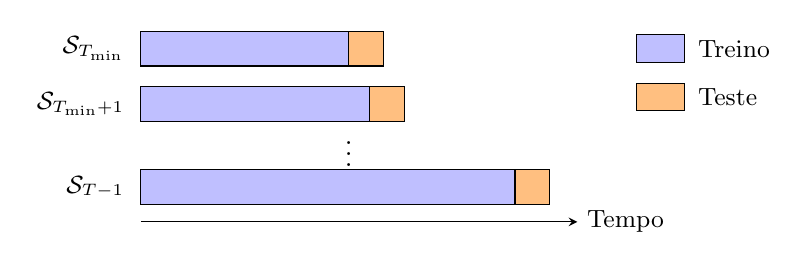
\begin{tikzpicture}[
  block/.style={draw, minimum height=0.45cm, inner sep=0},
  train/.style={block, fill=blue!25},
  test/.style={block,  fill=orange!50},
  scale=0.88
]
\node[left, font=\small] at (-0.1, 2.4) {$\mathcal{S}_{T_{\min}}$};
\node[left, font=\small] at (-0.1, 1.6) {$\mathcal{S}_{T_{\min}+1}$};
\node at (3.0, 1.0) {$\vdots$};
\node[left, font=\small] at (-0.1, 0.4) {$\mathcal{S}_{T-1}$};

\draw[train] (0,    2.15) rectangle (3.0,  2.65);
\draw[test]  (3.0,  2.15) rectangle (3.5,  2.65);

\draw[train] (0,    1.35) rectangle (3.3,  1.85);
\draw[test]  (3.3,  1.35) rectangle (3.8,  1.85);

\draw[train] (0,    0.15) rectangle (5.4,  0.65);
\draw[test]  (5.4,  0.15) rectangle (5.9,  0.65);

\draw[->, >=stealth] (0, -0.1) -- (6.3, -0.1) node[right, font=\small] {Tempo};
\node[draw, fill=blue!25,   minimum width=0.6cm, minimum height=0.35cm] at (7.5, 2.4) {};
\node[right, font=\small] at (7.9, 2.4) {Treino};
\node[draw, fill=orange!50, minimum width=0.6cm, minimum height=0.35cm] at (7.5, 1.7) {};
\node[right, font=\small] at (7.9, 1.7) {Teste};
\end{tikzpicture}
\caption{Protocolo \textit{walk-forward}: a janela de treinamento cresce incrementalmente e o modelo é avaliado apenas em dados futuros, respeitando a ordem das observações na divisão entre treino e avaliação.}
\label{fig:walkforward}
\end{figure}

Na Bahia, os prefixos de treino têm 17 e 23 ciclos, seguidos por sete de validação e sete de teste. As duas origens compartilham um ciclo de teste. Características, escalas e parâmetros usam somente o prefixo; a escolha usa a validação das demais lojas. O teste da loja reservada não participa dessas decisões.

O treinamento de controladores, a seleção de uma política e a avaliação da recomendação exigem papéis temporais separados. O primeiro ajusta parâmetros; o segundo usa validação para comparar candidatos; o último mede o resultado em demanda futura intocada. Avaliar o seletor com a mesma matriz que define seus rótulos mede ajuste retrospectivo. Mesmo a exclusão de uma loja da rotulagem não corrige informação futura já incorporada à calibração de suas políticas.

\subsection{Inferência e Unidade Experimental}

Wilcoxon compara pares de políticas nas mesmas séries; Friedman e Nemenyi comparam postos entre candidatos; tamanhos de efeito e diferenças absolutas descrevem relevância prática, conforme a Seção~\ref{sec:stat_tests}. Os testes usam nível nominal de 5\%, com procedimento de comparações múltiplas identificado na execução. Estratificações exploratórias não devem produzir muitas declarações isoladas de significância sem considerar sua multiplicidade.

A unidade de observação é a série loja--produto. Séries da mesma loja e lojas que compartilham produtos ou condições comerciais podem ser dependentes. A análise deve reconhecer essa estrutura, por exemplo, mediante reamostragem por loja e verificações de sensibilidade. Não se obtém independência multiplicando o número de séries por repetições determinísticas.

As três sementes estocásticas são promediadas dentro de cada caso série--origem e política antes da comparação. A reamostragem pareada preserva os produtos e origens de cada loja. Os intervalos são condicionais aos ajustes e escolhas fixos, sem retreinamento nos sorteios; por isso não representam toda a incerteza da investigação.

\section{Geração de Rótulos e PSE}
\label{sec:selecao_contextual}
\subsection{Problema de Seleção}

A formulação segue o problema de seleção de algoritmos de \citet{Rice1976AlgorithmSelection}: descrever uma instância e escolher uma alternativa do portfólio. A discussão de portfólios~\citep{Huberman1997AlgorithmPortfolios} motiva diversidade de candidatos. Os resultados de \citet{Wolpert1997NoFreeLunch} não demonstram que qualquer perfil específico melhorará decisões; a utilidade da representação precisa ser testada na população estudada.

O alvo conceitual é
\begin{equation}
\hat\pi_i^*=\arg\min_{\pi\in\Pi}\mathbb E[\mathrm{CTI}(\pi,i)]
\quad\text{sujeito a }\mathbb E[\mathrm{NS}(\pi,i)]\geq\alpha_{\min}.
\label{eq:policy_selector}
\end{equation}
Na matriz disponível, a esperança é aproximada pelo resultado registrado, não por uma distribuição comprovadamente estimada. O rótulo identifica a melhor candidata observada sob o limiar, não um ótimo universal. Se nenhuma atende ao serviço, registra-se inviabilidade; uma escolha pelo maior NS é apenas fallback, com o déficit informado.

Custos empatados devem receber regra estável, preferindo serviço e, depois, um identificador fixo. Quando diferenças são muito pequenas, um conjunto de candidatas equivalentes pode ser mais adequado que uma classe rígida. A estabilidade dos rótulos diante de sementes, custos e períodos é parte da validação: acurácia alta ao reproduzir rótulos arbitrários não garante melhora operacional.

\subsection{Treinamento e Avaliação Propostos}

O conjunto supervisionado reúne $(\phi(\mathbf d_i),\hat\pi_i^*)$. XGBoost é o classificador principal previsto~\citep{ChenGuestrin2016XGBoost}, com referência de 300 árvores, profundidade seis, taxa 0,05 e amostragem 0.8. LightGBM~\citep{Ke2017LightGBM} e RandomForest são alternativas. A presença dessas implementações e de artefatos de ajuste não equivale à validação do PSE em escala nacional ou em produção.

A avaliação deve separar lojas e períodos, evitando que produtos da mesma loja apareçam simultaneamente no treino e no teste sem justificativa. Validação estratificada pode ser usada quando todas as classes têm suporte suficiente, mas não resolve dependência entre instâncias. Classes raras exigem estratégia explícita; excluí-las da validação e depois reportar desempenho global de treino ocultaria seu efeito.

Acurácia balanceada, F1-macro e F1 ponderado ajudam a interpretar desbalanceamento, mas o resultado principal do seletor deve ser custo e serviço das políticas recomendadas. Uma classe incorreta pode ter desempenho praticamente igual ao rótulo, enquanto uma escolha correta pode não cumprir o serviço no futuro. A comparação deve incluir o melhor candidato global escolhido na mesma validação, EOQ com unidades consistentes e seleção sem a variável de perfil.

O estudo também precisa separar métricas após ajuste em toda a amostra das métricas fora do ajuste. Probabilidades do classificador não são probabilidades calibradas de viabilidade de serviço. A importância das características pode indicar associações, mas não prova causalidade nem estabilidade entre períodos. Essas verificações integram a continuidade do trabalho, descrita no Capítulo~\ref{cap:plano_continuidade}.

\subsection{Aplicação e Reavaliação}
\label{sec:aplicacao_aipe}

O produto previsto é uma política recomendada, um ranking de alternativas e um indicador de incerteza. Quando disponíveis, custos e serviços simulados acompanham a decisão como evidência condicionada ao cenário. Recomendações incertas ou inviáveis exigem nova análise; um limiar de confiança, como 0,50, é uma regra de triagem a calibrar, não comprovação de que o risco esteja controlado.

A adaptação proposta consiste em recalcular características e consultar o seletor em intervalos definidos, por exemplo a cada seis ciclos. Essa consulta não equivale a retreinar o modelo, e não há evidência de implantação contínua dessa rotina nos experimentos apresentados. Uma aplicação real também depende de disponibilidade da política no sistema, restrições empresariais e monitoramento do serviço realizado.

\section{Escopo Experimental e Rastreabilidade}
\label{sec:protocolo_exp}
\label{sec:reporting}

A Bahia reúne 145 séries em 115 lojas e nove produtos, com duas origens e 4.350 ajustes completos. O M5 utiliza uma coorte de 2.408 identificadores, com elegibilidade própria em cada prefixo, e permanece em execução. As bases são analisadas separadamente sob perguntas e critérios comuns. A expansão nacional foi retirada da execução ativa.

Cada execução deve associar dados, lista de políticas, parâmetros, semente, divisão temporal e versão do código. Arquivos de características, perfis, KPIs e recomendações têm funções diferentes; o relatório precisa indicar qual foi usado em cada tabela. Hashes de entrada e manifesto de execução ajudam a detectar troca de arquivos, mas não certificam, isoladamente, ausência de informação futura ou fidelidade do algoritmo.

O Apêndice~\ref{app:reproducibility} concentra os parâmetros da avaliação e sua rastreabilidade. Dados, fontes de conhecimento e versões de desenvolvimento são preservados no projeto, sem compor matrizes paralelas na síntese dos resultados.

O Capítulo~\ref{cap:results} responde às perguntas com a cobertura disponível, distinguindo evidência completa de análises ainda pendentes. A execução M5 só sustentará conclusões após conferência de sua matriz.